%*************************************************************
\chapter{CSCW \& Design}\label{ch:CSCWDesign}
%*************************************************************

	Der Begriff >>Computer Supported Cooperative Work<< (CSCW) bezeichnet ein multidisziplinäres Forschungsgebiet, das die kooperative Zusammenarbeit mehrerer Gruppen untersucht und Technologien zur Unterstützung selber entwickel. CSCW existiert seit den frühen achtziger Jahren. Um herauszufinden, wie die Technik Menschen bei ihrer Zusammenarbeit unterstützen kann, organisierten Irene Greif und Paul Cashman im Jahre 1984 einen Workshop für Personen, die sich mit der Arbeitsweise von Menschen auseinandersetzten \citep{Grudin:1994}. Unter diesen Personen befanden sich Spezialisten aus verschiedenen wissenschaftlichen Bereichen, wie zum Beispiel Ökonomie, Sozialpsychologie, Anthropologie, Ethnologie und Pädagogik. Dieser Workshop war der Versuch der Techniker, Teamarbeit besser zu verstehen, um folglich unterstützende Technologien entwickeln zu können \citep{Grudin:1994, Rama:2006p245}. Seither hat CSCW sich zu einem nahezu riesigen wissenschaftlichen Forschungsgebiet entwickelt, dem sich heute unzählige Experten widmen. Trotzdem sind sich die Wissenschaftler nicht immer ganz einig bei der Definition des Begriffes CSCW. Die Bedeutung von >>Cooperative Work<< erscheint nicht eindeutig und führt häufig zu unterschiedlichen Interpretation seitens wissenschaftlicher Autoren \citep{Gerlicher:2007p241}. Einige setzen >>Cooperation<< gleich mit >>Collaboration<<, andere hingegen unterscheiden die beden Begriffe sehr strikt. Dillenbourg et al. definieren die Begriffe beispielsweise so: 
	
	\medskip\begin{quote}{>>Cooperation and collaboration do not differ in terms of whether or not the task is distributed, but by virtue of the way in which it is divided; in cooperation the task is split (hierarchically) into independent subtasks; in collaboration cognitive processes may be (heterarchically) divided into intertwined layers. In cooperation, coordination is only required when assembling partial results, while collaboration is “...„ a coordinated, synchronous activity that is the result of a continued attempt to construct and maintain a shared conception of a problem.<<} \citep{Dillenbourg:1995} \end{quote}
	
	\medskip Die beiden Begriffe unterscheiden sich also nicht darin ob Arbeit auf mehrere Individuen aufgeteilt wird oder nicht, sondern in der Art und Weise, wie sie aufgeteilt wird. Bei >>Cooperation<< wird die Arbeit in einzelne, unabhängige Module aufgeteilt, die zuerst abgewickelt und danach wieder zu einem Ganzen zusammengesetzt werden können. >>Collaboration<< hingegen ist eine koordinierte, synchrone Aktivität und resultiert aus dem fortwährenden Versuch, eine gemeinsame Auffassung eines Problems zu konstruieren und zu erhalten.
	
	In dieser Arbeit werden die beiden Begriffe synonym verwendet, da sich beide aus dem Englischen als >>Zusammenarbeit<< übersetzen lassen.
	
	\bigskip Die Erkenntnisse, die bei der Erforschung von CSCW gewonnen werden verwendet man dazu, sinnvolle >>Groupware<< zu konzipieren. Groupware bezeichnet also die technische, praktische Umsetzung, die auf den Theorien des CSCW basiert. Alle Systeme, Applikationen und Werkzeuge, die CSCW unterstützen, können somit unter dem Begriff Groupware zusammengefasst werden \citep{Koch2008, Gerlicher:2007p241}. Häufig werden diese Systeme auch als >>kollaborative Software<< bezeichnet \citep{Bannon:1990p244}. Gerlicher und Ansgar definieren Groupware wie folgt:
	
	\medskip\begin{quote}{>>Der Begriff Groupware bezeichnet ein aus Software und eventuell spezifischer Hardware bestehendes System, das die Zusammenarbeit im Team durch die Schaffung von Kommunikations- und/oder Koordinationslösungen unterstützt oder ermöglicht.<< \citep{Gerlicher:2007p241}}\end{quote}
	
	

\begin{itemize}
	\item {CSCW: four characters in search of a context}
	\item {CSCW an Enterprise 2.0 - towards an integrated perspective}
	\item {A survey and comparison of CSCW groupware applications}
	\item {CSCW - kollaborative Systeme und Anwendungen}
\end{itemize}

\section{Klassifikation von CSCW}


\begin{figure}[bth]
	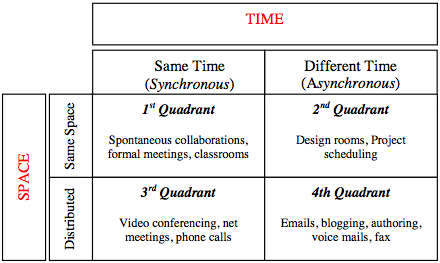
\includegraphics[width=\textwidth]{gfx/ramaCSCWQuadranten.png}
	\caption{Rama und Bishop \citep{Rama:2006p245} illustrieren in dieser Grafik die Unterteilung von CSCW in vier Kategorien, die sich durch ihre räumlichen und zeitlichen Eigenschaften unterscheiden. Der Faktor Zeit definiert, ob Zusammenarbeit in einer Gruppe synchron oder asynchron passiert und der Faktor Raum definiert, ob sie am selben oder an geographisch distanzierten Orten passiert.}
	\label{fig:ramaCSCW}
\end{figure}


\subsection{Asynchrone Systeme}

Unter asynchroner Groupware versteht man Systeme, die keine Echtzeitanforderungen erfüllen müssen. Das bedeutet, dass die Nutzung dieser Systeme im Normalfall zeitversetzt erfolgt. Die wohl bekannteste asynchrone Groupware Anwendung ist die digitale Übermittlung von Textnachrichten in Form einer \emph{E-Mail}. Diese Nachrichten können an und von mehreren Personen versendet, empfangen und weitergeleitet werden. Dabei müssen Absender und Empfänger nicht gleichzeitig online sein, denn die \emph{E-Mail} kann zu jedem beliebigen Zeitpunkt vom Empfänger abgerufen werden.

Eine andere, jedoch der \emph{E-Mail} sehr ähnliche Form asynchroner Groupware sind \emph{Newsgroups und Mailinglisten} \citep{Gerlicher:2007p241}. Sie dienen dem Nachritenaustausch in einer größeren Gruppe an Benutzern. \emph{Newsgroups} zeigen Nachrichten nur dann an, wenn ein Benutzer diese direkt anfordert, \emph{Mailinglisten} hingegen werden automatisch an all jene Personen weitergeleitet, welche die entsprechende Liste abonniert haben.

Auch \emph{Workflow-Management Systeme} werden von Gerlicher und Ansgar \citep{Gerlicher:2007p241} zur asynchronen Groupware gezählt, da sie die Arbeit unterschiedlicher Personen in einer Organisation regeln. Sie dienen der Steuerung arbeitsteiliger Prozesse und man bezeichnet sie auch Geschäftsprozess-Management-Systeme.

Das World Wide Web (WWW) ist ein \emph{Hypertext-basiertes System} und gehört ebenfalls zur asynchronen Groupware \citep{Gerlicher:2007p241}, da es einer sehr großen Anzahl an Personen ermöglicht, auf digitalem Wege Informationen auszutauschen. \emph{Hypertext-basierte Systeme} nutzen das Internet oder ein bestimmtes Intranet, um ihre Dienste über einen Webbrowser zugänglich zu machen. Solch eine Webschnittstelle kann prinzipiell für fast jede Art der asynchronen Groupware implementiert werden. 

Schlussendlich nennen Gerlicher und Ansgar noch Gruppenkalender als asynchrones Groupware System. Der Gruppenkalender ist ein Tool, das sehr häufig in größeren Unternehmen eingesetzt wird. Er ermöglicht die Terminplanung und Koordination von vielen Personen. Terminkonflikte werden automatisch erkannt und das System kann eigenständig jene Zeiträume finden, zu denen jeder erforderliche Teilnehmer eines Meetings frei zur Verfügung steht. Dies setzt jedoch eine gute Datenpflege aller Benutzer voraus und wird teilweise als unangenehmer Eingriff in die Privatsphäre empfunden \citep{Gerlicher:2007p241}.

\subsection{Synchrone Systeme}

Dem gegenüber stehen synchrone Groupware Systeme, die sich dadurch charakterisieren, dass Benutzer zeitgleich auf Daten und Informationen zugreifen \citep{Gerlicher:2007p241}. Ein Beispiel dafür sind elektronische Tafeln, denn sie erlauben mehreren Nutzern, die sich an unterschiedlichen Orten befinden, auf eine für alle sichtbare Fläche zu zeichnen. Häufig werden solche Tafeln bei Besprechungen eingesetzt, bei denen die Teilnehmer nicht im selben Raum sind. Dadurch wird es möglich, Konzepte und Ideen besser zu kommunizieren und für die anderen greifbarer zu machen.

\emph{Application Sharing Systeme} zählen ebenfalls zur synchronen Groupware und gestatten das Teilen von Drittapplikationen mit anderen Personen \citep{Gerlicher:2007p241}. Man bezeichnet diese Anwendungen im Englischen auch als \emph{Remote Desktop}\footnote{Zu Deutsch: Entfernter Schreibtisch. Gemeint ist damit die virtuelle Schreibtischfläche des Betriebssystems.}. Dadurch wird es möglich, mit geografisch distanzierten Kollegen an jedem beliebigen Programm zu kooperieren. Beide Benutzer sehen die Applikation, die auf einem der Computer läuft und können mit ihr interagieren. 

Weitere synchrone Systeme sind Video- und Multimediale Konferenzsysteme \citep{Gerlicher:2007p241}. Erstere übertragen Video und Audio an mehrere verteilte Computer und werden eingesetzt, um virtuelle Meetings abzuhalten. Die Teilnehmer befinden sich meist an verschiedenen Orten und können so fast genauso kommunizieren, als würden sie sich in einem Raum befinden. Letztere bieten zusätzlich die Möglichkeit, multimediale Inhalte (beispielsweise Präsentationen) an die Teilnehmer der Konferenz zu übertragen. Systeme zu Entscheidungsfindung sind oft ein integraler Bestandteil solcher Software und bieten Werkzeuge für Ideenfindung und Brainstorming. Über auf diesem Wege generierte Konzepte kann dann abgestimmt und so die Spreu vom Weizen getrennt werden. 

\emph{Chat-Systeme}, ebenfalls der synchronen Groupware zuzuordnen, sind weitgehend bekannt und werden sehr häufig eingesetzt. Benutzer können durch diese Anwendungen in Echtzeit untereinander Textnachrichten austauschen und so eine Konversation führen, als säßen sie sich gegenüber. 

\subsection{Multisynchrone Systeme}

Versionsverwaltungssysteme werden von Gerlicher und Ansgar als multisynchrone Systeme definiert \citep{Gerlicher:2007p241}. Häufig werden diese in Softwareprojekten und auch bei der Erstellung von umfangreichen Dokumenten, beispielsweise Büchern eingesetzt. Das System übernimmt die Verwaltung der Dateien und sichert die Konsistenz der Daten. Es wird dadurch möglich, dass mehrere Personen gleichzeitig an der selben Datei arbeiten. Tatsächlich haben aber alle Benutzer eine eigene Kopie der Datei und das System synchronisiert die Dateien selbständig. Ein weiterer großer Vorteil von Versionsverwaltungssystemen, ist die Nachvollziehbarkeit von Änderungen \citep{Gerlicher:2007p241} an einzelnen Dateien. Das System legt für jede neue Version einer Datei ein Backup ab, das zu einem späteren Zeitpunkt bei Bedarf wiederhergestellt werden kann. Es ist zu jedem Zeitpunkt klar, wer welche Änderungen an einer bestimmten Datei durchgeführt hat. 

\bigskip Es wird deutlich, dass CSCW und Groupware sehr weitläufig sind und viele verschiedene Bereiche betreffen. Daher ist es bis heute immer noch eine große Herausforderung geblieben, bedienbare, effiziente und intuitive Systeme zu entwickeln, die die Arbeit der Benutzer tatsächlich optimieren und keinen Mehraufwand verursachen. Im folgenden Abschnitt widmen wir uns den Problemfeldern, die damit zusammenhängen.

\section{Wichtige Aspekte bei Design von Groupware}
\begin{itemize}
	\item {Helping CSCW Applications Succeed: The Role of Mediators in the Context of Use}
	\item {How Can Human and Design Sciences Cooperate in CSCW?}
	\item {CSCW as a basis for interactive design semantics}
	\item {Developing CSCW Tools for Idea Finding - Empirical Results and Implications for Design}
	\item {Design for Design: Support for Creative Practice in CSCW in Design}
	\item {Anforderungen an interaktive Kooperationslandschaften für kreatives Arbeiten und erste Realisierungen}
	\item {Making Sense of Collaboration: The Challenge of Thinking Together in Global Design Teams}
	\item {Single Display Groupware: A Model for Co-present Collaboration}
	\item {Synergy: A Prototype Collaborative Environment to Support the Conceptual Stages of the Design Process}
	\item {Architecture of BEACH: The Software Infrastructure for Roomware Environments}
	\item {A Multiple Device Approach for Supporting Whiteboard-based Interactions}
	\item {Avoiding Interference: How People use Spatial Separation and Partitioning in SDG Workspaces}
	\item {Being Here: Designing for Distributed Hands-On Collaboration in Blended Interaction Spaces}
	\item {Beyond the Chalkboard: Computer Support for Collaboration and Problem Solving in Meetings}
\end{itemize}

\section{Probleme in Design und Evaluierung von Groupware}

In seiner Studie über die Schwierigkeit des Designs und der Evaluierung von Groupware \citep{Grudin:1988p126}, nennt Jonathan Grudin drei grundlegende Problemfelder:

\begin{itemize}
	\item
	Das Missverhältnis zwischen denen, die einen zusätzlichen Aufwand betreiben müssen und jenen die einen tatsächlichen Nutzen haben
	\item
	Das Treffen von Entscheidungen durch leitende Personen, basierend auf ihrer Intuition
	\item
	Das Unterschätzen der Schwierigkeiten, die mit einer Evaluierung von CSCW-Systemen verbunden sind
\end{itemize}

Am Beispiel einer Software zur automatischen Planung von Sitzungen zeigt Grudin wie ein ungleiches Verhältnis zwischen einzelnen Nutzern einer Groupware entstehen kann. 

Wenn ein Mitarbeiter eine Sitzung mit anderen vereinbaren möchte, so muss er der Software nur die gewünschten Teilnehmer mitteilen. Das Programm vergleicht dann eigenständig die elektronischen Kalender dieser Personen und bucht einen Termin zu jener Zeit, in der noch alle Teilnehmer frei sind. Voraussetzung hierfür ist dementsprechend, dass jeder Mitarbeiter im Unternehmen einen elektronischen Kalender führt. Jene Personen, die in leitenden Positionen tätig sind, führen sehr wahrscheinlich einen Kalender oder haben eine Sekretärin, die diese Aufgabe übernimmt. Probleme ergeben sich dann, wenn leitende Mitarbeiter Termine mit Angestellten vereinbaren möchten, da diese häufig keinen elektronischen Kalender führen. Das System glaubt daher, dass ein Termin zu jeder Zeit möglich wäre und bucht unter Umständen einen ungünstigen Zeitpunkt für entsprechende Teilnehmer. \graffito{Groupware muss so konzipiert werden, dass jeder Benutzer einen Nutzen hat und zusätzliche Aufwände so gering wie möglich ausfallen.} Um dieser Problematik vorzubeugen, müssten alle Mitarbeiter, vom einfachen Angestellten bis hin zum Geschäftsführer, einen elektronischen Kalender führen. Angestellte hätten dadurch einen zusätzlichen Aufwand, jedoch wenig bis gar keinen Nutzen vom System. Dieser Umstand kann sehr leicht dazu führen, dass die Software in der Praxis keine Akzeptanz unter den Benutzern findet und dadurch scheitert.

\medskip Beim Design von multi-user Software verlassen sich laut Butler et al. \citep{ButlerK:1987} Entscheidungsträger häufig auf ihre Intuition, die wiederum auf persönlichen Erfahrungen, zumeist im single-user Bereich, beruht. Es mag relativ einfach sein, ein Gespür dafür zu entwickeln, wie gut die >>User Experience<<\footnote{User Experience bezeichnet das Nutzungserlebnis, das eine Person empfindet, während sie ein Produkt, einen Service, eine Software, etc. benutzt, bzw. in Anspruch nimmt. Ziel des User Experience Designs ist es, dieses Anwendungserlebnis für den Benutzer möglichst angenehm und positiv zu gestalten und all seine Erwartungen zu erfüllen.} eines Textverarbeitungs- oder Tabellenkalkulationsprogramm ausfällt, jedoch wird Groupware von einem breiten Spektrum an Personen verwendet und alle diese Benutzer haben unterschiedliche Hintergründe und Berufe, ungleiches technisches Know-How und abweichende Zugänge zum Programm. Die Software wird sehr wahrscheinlich scheitern, wenn die Intuition der Entscheidungsträger die Komplexität ignoriert, die durch solch eine Gruppendynamik zustande kommt. 

Die von Grudin \citep{Grudin:1988p126} angeführte Software zur automatischen Planung von Sitzungen bezeichnet er selbst als anfällig für ein solches Scheitern durch falsche Intuition von leitenden Mitarbeitern. Er begründet dies so, dass jene leitenden Mitarbeiter selbst mit großer Wahrscheinlichkeit bereits einen elektronischen Kalender führen und daher vordergründig nur den eigenen Nutzen erkennen. Mangelnde Empathie kann zu Folge haben, dass der zusätzliche Aufwand, der einfachen Angestellten entsteht, nicht berücksichtigt wird. 

\medskip Die Evaluierung von Groupware erfordert eine spezielle Vorgangsweise, basierend den Methodiken der Psychologie und Anthropologie \citep{Grudin:1988p126}. Laut Grudin fehlen diese Fähigkeiten zum Zeitpunkt der Untersuchung (1988) in den meisten Entwicklungs- und Forschungsteams, da qualifizierte Personen aus den Bereichen >>Human Factors Engineering\footnote{Als Human Factors Engineering bezeichnet man jene Disziplin, die sich mit den Fähigkeiten und Grenzen des Menschen beschäftigt und diese Erkenntnisse auf das Design von Produkten, Prozessen, Systemen und Arbeitsplätzen anwendet. Dazu gehört das Überprüfen auf >>Usability<<, das Erstellen von Nutzerprofilen und die Entwicklung von Benutzerdokumentation und Trainingsprogrammen.} und kognitiver Psychologie noch selten vertreten sind. Zusätzlich ist der mit der Evaluierung verbundene zeitliche und finanzielle Aufwand erheblich höher, da immer ganze Gruppen an Probanden getestet werden müssen.

\medskip Im Anbetracht dieser, von Grudin schon sehr früh erkannten Problemfelder, erörtern wir im nächsten Kapitel eine Studie, die vier verschiedene Konzepten zum Vorschein gebracht hat, welche durch und durch Benutzer und nicht vorrangig Technologien berücksichtigen.

\section{Warum Groupware unseren Erwartungen oft nicht gerecht wird}
\begin{itemize}
	\item {The Productivity Paradox: Why hasn't Information Technology Fulfilled its Promise?}
	\item {Why CSCW Applications Fail: Problems in the Design and Evaluation of Organizational Interfaces}
\end{itemize}

\section{Der positive Nutzen von gut umgesetzter Groupware}

\section*{Zusammenfassung}
lorem ipsum
